\documentclass[conference]{IEEEtran}
\usepackage{amsmath,amssymb,booktabs,graphicx,url}
\usepackage[hidelinks]{hyperref}
\usepackage{tikz}
\usetikzlibrary{arrows.meta,positioning}
\usepackage{placeins}
\graphicspath{{../figures/}}
\title{Cross-Institution Reliability of Temporal Attributions in Network Traffic Forecasting}
\author{\IEEEauthorblockN{Anonymous research draft}\IEEEauthorblockA{Expanded empirical draft, 7 November 2026; authors and venue to be finalized}}
\begin{document}\maketitle
\begin{abstract}
A traffic forecaster can transfer to a new institution without establishing that its temporal explanations remain useful. We audit this distinction using CESNET-TimeSeries26: an initial study of 32 source, eight validation and eight unseen target institutions, followed by a separately frozen cohort of 32 newly evaluated targets using the same source anchors and locked models. Ridge, DLinear and gated recurrent forecasters predict one- and six-hour traffic endpoints from one week of history. We separate forecast error, numerical attribution checks and ranking alignment under two controlled history replacements. The original prespecified one-hour GRU Shapley contrast is $-0.0189$ with a nominal 95\% interval of $[-0.0891,0.0533]$ across seven complete pairs. The new-cohort contrast is $-0.0075$, interval $[-0.0402,0.0241]$, across 30 complete pairs. Neither establishes systematic degradation or equivalence. The original reference-specific zero-excluding secondary pattern does not recur in the new cohort. A prespecified nested 16-to-64-origin comparison and alternative uncertainty procedures expose sampling assumptions. The expansion also reveals extreme relative forecast errors on near-constant low-volume traffic and undefined ranking games; numerical validity and an informative complete-pair mean do not certify those regimes. These results support an auditable, reference-explicit empirical benchmark with explicit exclusions and bounded within-network conclusions.
\end{abstract}
\begin{IEEEkeywords}network traffic forecasting, explainability, institution transfer, temporal attribution, evaluation\end{IEEEkeywords}

\section{Introduction}
Network traffic forecasting supports resource planning, but a forecast and an explanation answer different operational questions. Forecast error measures agreement with subsequent observations. A temporal attribution distributes a prediction contrast over historical inputs. A ranking test measures how an ordering responds to a specified intervention on those inputs. Success on one does not certify the others. This distinction becomes consequential when a pooled forecaster is deployed to an institution absent from model fitting.

Transferable traffic prediction is established research: TransMUSE studies transfer across edge cohorts~\cite{transmuse}. Network forecasting explanations and their operational use are also established, including AIChronoLens~\cite{aichrono}. More recent work studies explanation generalization for time series~\cite{timesae}. Accordingly, the question here is narrower than whether transfer or explainable forecasting is possible: under a fixed, institution-disjoint network deployment protocol, what evidence supports the reliability of temporal attribution rankings, and how does that evidence depend on the attribution contrast and measurement operator?

We use a public multi-year traffic dataset~\cite{cesnet26,dataset}. We retain source-only fitting, unseen validation institutions, fixed target institutions, timestamp-matched explanation cases, repeated neural seeds, and a prespecified primary comparison. After the initial eight-target experiment, we freeze a further 32-target cohort before its scoring, retaining the same source anchors and checkpoints. This expands the project to 80 unique institutions within one ISP; it does not provide independent networks or a new training run. Our contribution is an empirical audit design and its executed evidence, rather than a new attribution algorithm. Specifically, we provide (i) a reproducible institution-disjoint benchmark with explicit missingness and effective sample counts; (ii) separate checks of numerical attribution behavior and controlled-operator ranking alignment; and (iii) a paired transfer estimate with reference, horizon, model, and bias-calibration analyses clearly designated as secondary; and (iv) an executed new-target within-network replication with prespecified timestamp-density and uncertainty sensitivities.

Both cohort primary results are inconclusive about systematic ranking degradation. The stronger nominal original secondary pattern under a different attribution reference does not recur as a zero-excluding interval in the larger cohort. We report the original and new outcomes separately, including the informative-case exclusions and low-volume forecast failures.

Figure~\ref{fig:pipeline} summarizes the data flow, deployment arms, and three distinct evaluation branches.

\begin{figure*}[t]\centering
\resizebox{\textwidth}{!}{% Editable vector pipeline; input from paper.tex inside a figure*.
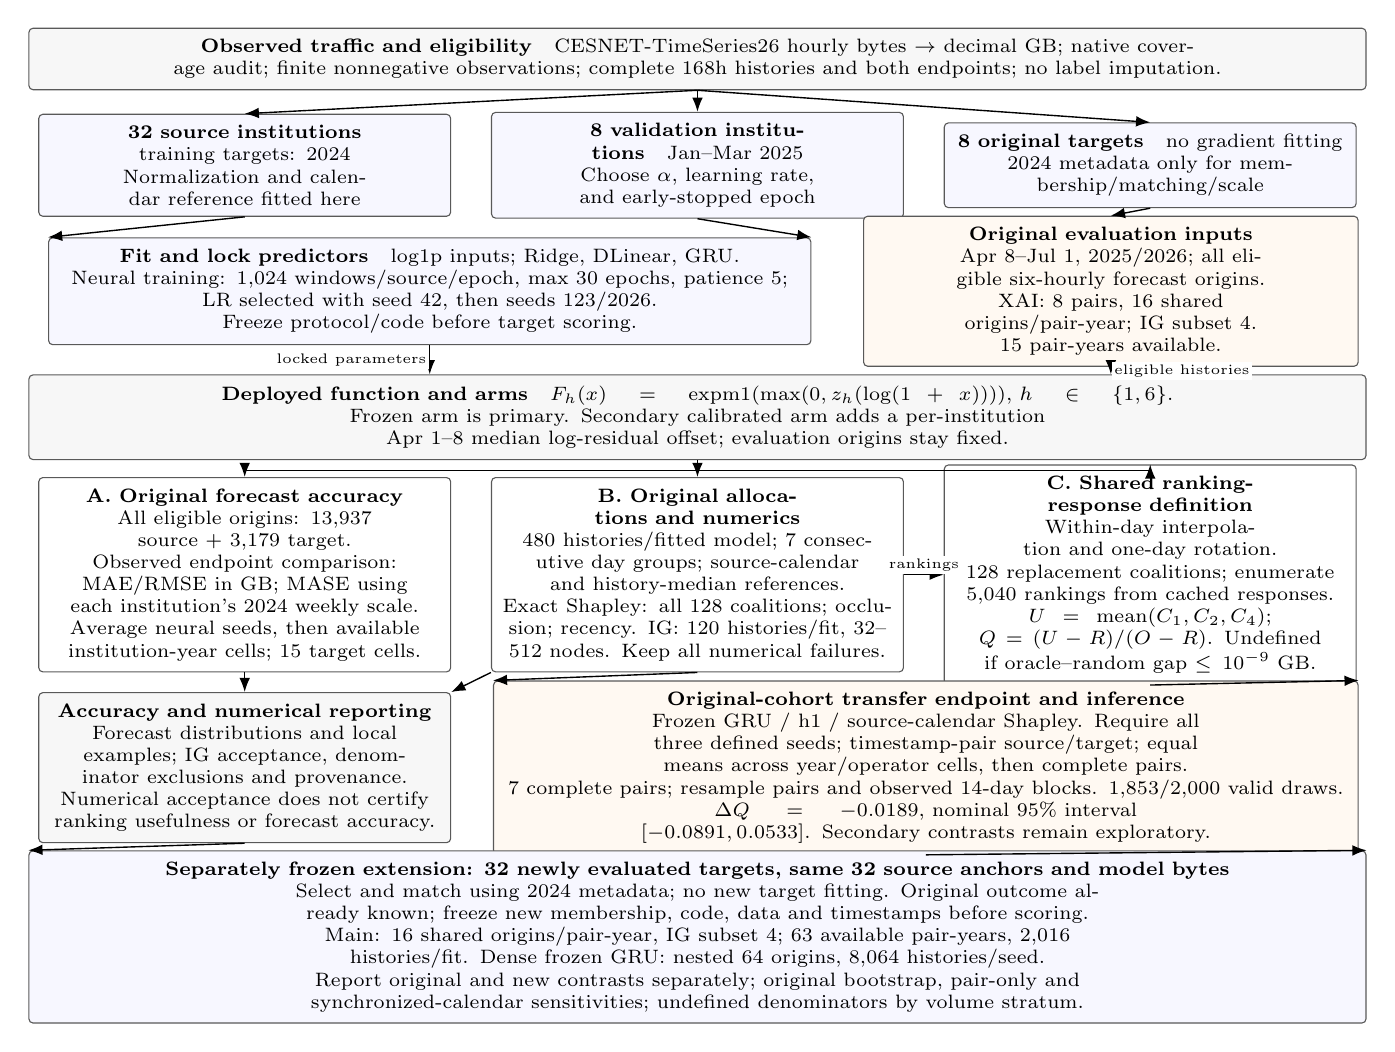
\begin{tikzpicture}[
  font=\scriptsize, x=1cm,y=1cm,
  box/.style={draw=black!65,rounded corners=1.5pt,align=center,inner sep=4pt},
  cohort/.style={box,text width=4.95cm,minimum height=.93cm,fill=blue!3},
  lane/.style={box,text width=4.95cm,minimum height=1.98cm},
  arr/.style={-{Latex[length=1.8mm]},line width=.5pt},
  tag/.style={font=\tiny,fill=white,inner sep=1pt}
]
\node[box,text width=16.7cm,minimum height=.75cm,fill=black!3] (data) at (0,0)
{\textbf{Observed traffic and eligibility}\quad CESNET-TimeSeries26 hourly bytes $\to$ decimal GB; native coverage audit; finite nonnegative observations; complete 168h histories and both endpoints; no label imputation.};
\node[cohort] (source) at (-5.75,-1.35) {\textbf{32 source institutions}\quad training targets: 2024\\Normalization and calendar reference fitted here};
\node[cohort] (val) at (0,-1.35) {\textbf{8 validation institutions}\quad Jan--Mar 2025\\Choose $\alpha$, learning rate, and early-stopped epoch};
\node[cohort] (target) at (5.75,-1.35) {\textbf{8 original targets}\quad no gradient fitting\\2024 metadata only for membership/matching/scale};
\foreach \a in {source,val,target}\draw[arr] (data.south)--(\a.north);
\node[box,text width=9.4cm,minimum height=1.13cm,fill=blue!3] (fit) at (-3.4,-2.95)
{\textbf{Fit and lock predictors}\quad log1p inputs; Ridge, DLinear, GRU.\\Neural training: 1,024 windows/source/epoch, max 30 epochs, patience 5;\\LR selected with seed 42, then seeds 123/2026. Freeze protocol/code before target scoring.};
\node[box,text width=6.0cm,minimum height=1.13cm,fill=orange!5] (cases) at (5.25,-2.95)
{\textbf{Original evaluation inputs}\\Apr 8--Jul 1, 2025/2026; all eligible six-hourly forecast origins.\\XAI: 8 pairs, 16 shared origins/pair-year; IG subset 4.\\15 pair-years available.};
\draw[arr] (source.south)--(fit.north west);
\draw[arr] (val.south)--(fit.north east);
\draw[arr] (target.south)--(cases.north);
\node[box,text width=16.7cm,minimum height=.91cm,fill=black!3] (function) at (0,-4.55)
{\textbf{Deployed function and arms}\quad $F_h(x)=\operatorname{expm1}(\max(0,z_h(\log(1+x))))$, $h\in\{1,6\}$.\\Frozen arm is primary. Secondary calibrated arm adds a per-institution Apr 1--8 median log-residual offset; evaluation origins stay fixed.};
\draw[arr] (fit.south)--node[tag,left] {locked parameters}(function.north -| fit.south);
\draw[arr] (cases.south)--node[tag,right] {eligible histories}(function.north -| cases.south);
\node[lane] (forecast) at (-5.75,-6.55)
{\textbf{A. Original forecast accuracy}\\All eligible origins: 13,937 source + 3,179 target.\\Observed endpoint comparison: MAE/RMSE in GB; MASE using each institution's 2024 weekly scale.\\Average neural seeds, then available institution-year cells; 15 target cells.};
\node[lane] (attr) at (0,-6.55)
{\textbf{B. Original allocations and numerics}\\480 histories/fitted model; 7 consecutive day groups; source-calendar and history-median references.\\Exact Shapley: all 128 coalitions; occlusion; recency. IG: 120 histories/fit, 32--512 nodes. Keep all numerical failures.};
\node[lane] (response) at (5.75,-6.55)
{\textbf{C. Shared ranking-response definition}\\Within-day interpolation and one-day rotation.\\128 replacement coalitions; enumerate 5,040 rankings from cached responses.\\$U=\operatorname{mean}(C_1,C_2,C_4)$; $Q=(U-R)/(O-R)$. Undefined if oracle--random gap $\leq10^{-9}$ GB.};
\draw[arr] (function.south)--(0,-5.23)--(-5.75,-5.23)--(forecast.north);
\draw[arr] (function.south)--(attr.north);
\draw[arr] (function.south)--(0,-5.23)--(5.75,-5.23)--(response.north);
\draw[arr] (attr.east)--node[tag,above] {rankings}(response.west);
\node[box,text width=4.95cm,minimum height=1.5cm,fill=black!3] (audit) at (-5.75,-9.0)
{\textbf{Accuracy and numerical reporting}\\Forecast distributions and local examples; IG acceptance, denominator exclusions and provenance.\\Numerical acceptance does not certify ranking usefulness or forecast accuracy.};
\node[box,text width=10.7cm,minimum height=1.5cm,fill=orange!5] (infer) at (2.9,-9.0)
{\textbf{Original-cohort transfer endpoint and inference}\\Frozen GRU / h1 / source-calendar Shapley. Require all three defined seeds; timestamp-pair source/target; equal means across year/operator cells, then complete pairs.\\7 complete pairs; resample pairs and observed 14-day blocks. 1,853/2,000 valid draws.\\$\Delta Q=-0.0189$, nominal 95\% interval $[-0.0891,0.0533]$. Secondary contrasts remain exploratory.};
\draw[arr] (forecast.south)--(audit.north);
\draw[arr] (attr.south west)--(audit.north east);
\draw[arr] (attr.south)--(infer.north west);
\draw[arr] (response.south)--(infer.north east);

\node[box,text width=16.7cm,minimum height=1.37cm,fill=blue!3] (replicate) at (0,-11.15)
{\textbf{Separately frozen extension: 32 newly evaluated targets, same 32 source anchors and model bytes}\\Select and match using 2024 metadata; no new target fitting. Original outcome already known; freeze new membership, code, data and timestamps before scoring.\\Main: 16 shared origins/pair-year, IG subset 4; 63 available pair-years, 2,016 histories/fit. Dense frozen GRU: nested 64 origins, 8,064 histories/seed.\\Report original and new contrasts separately; original bootstrap, pair-only and synchronized-calendar sensitivities; undefined denominators by volume stratum.};
\draw[arr] (infer.south)--(replicate.north east);
\draw[arr] (audit.south)--(replicate.north west);
\end{tikzpicture}
}
\caption{Overall executed pipeline, including fitting/validation separation, both deployment arms, eligible future inputs, distinct accuracy/numerical/ranking branches, references and operators, case-selection budgets, the prespecified inferential unit, and the separately frozen new-target extension. The hash freeze is a local audit trail, not external preregistration. Replacement responses are controlled diagnostics, not identified causal demand effects.}\label{fig:pipeline}
\end{figure*}

\section{Related Work and Scope}
\subsection{Forecasting and network explanations}
TransMUSE~\cite{transmuse} addresses service-aware model transfer and prediction performance. DLinear~\cite{dlinear} demonstrates the importance of simple linear forecasting baselines, motivating their inclusion alongside a GRU~\cite{gru}. CESNET's comparative forecasting work~\cite{comparison} and the CESNET-TimeSeries26 descriptor~\cite{cesnet26} motivate evaluation across institutions and time. Our compact model set is a controlled benchmark, not an exhaustive assessment of current forecasting architectures.

AIChronoLens~\cite{aichrono} relates explanations to temporal properties and forecast errors in mobile networks. Explanations of aggregated network predictors have also been studied~\cite{aggregated}, as have attacks on explainability in networking~\cite{deexp}. The present study does not introduce temporal explanation, aggregation analysis, error repair, or adversarial robustness. Its focus is a fixed source-to-unseen-institution comparison on institutional byte-volume series.

\subsection{Attribution semantics and evaluation}
Integrated gradients (IG) explains a path-dependent prediction contrast~\cite{ig}; Shapley attribution allocates a coalition game~\cite{shap}. Baseline choice changes the question being answered~\cite{manyshap,baselines}. Different nonlinear allocations therefore need not agree, and an efficiency identity alone cannot establish the substantive correctness of an explanation. Sanity checks~\cite{sanity}, learned perturbations~\cite{perturb}, and InterpretTime~\cite{interprettime} further motivate examining the evaluation procedure itself.

TIMING~\cite{timing} discusses opposing signed effects, temporal paths, and cumulative response metrics. We use a cumulative absolute sequential response, with an explicitly defined normalization; cancellation awareness is not claimed as new. TimeSAE~\cite{timesae}, accepted at ICML 2026, already examines explanation generalization under shift. Our study differs in deployment unit, observed institutional traffic, input-day groups, and a numerical-versus-ranking audit. We do not implement or claim to outperform TimeSAE, TIMING, or other specialized explainers. The novelty claim is thus a bounded combination of experimental controls and empirical evidence in this network setting, subject to further venue-specific literature review.

\section{Data and Frozen Deployment Protocol}
\subsection{Provenance and eligibility}
We use the official hourly institutional \texttt{n\_bytes} files from CESNET-TimeSeries26, Zenodo record 21945629, under CC BY 4.0~\cite{dataset}. The dataset covers institutions within the CESNET3 network~\cite{cesnet26}; institutions are not independent ISPs. We verified the downloaded archive checksum, source-member SHA-256 values, and hashes of all 48 derived files. Traffic units are decimal GB ($10^9$ bytes). No attack-detection labels or synthetic traffic mixtures enter this benchmark.

Native time mappings identify hourly coverage. A usable hour has six native ten-minute records and an observed finite nonnegative value. We require all 168 historical hours and both forecast endpoints to be usable. We retain observed zeros, do not impute labels, and do not convert absent values into zeros. A conservative global flag excludes windows crossing 21 May--4 June 2024 because of a documented probe-artifact concern; its institution-specific scope is uncertain. This screening choice is not evidence that every institution was affected.

Twelve institutions used in earlier development are excluded from this study's membership. Among the remaining eligible institutions, four 2024 median-volume strata and deterministic SHA-256 ordering select 48 institutions: 32 source, eight validation, and eight target. Selection uses saved 2024 coverage and volume metadata, not final forecasting or attribution results. Eight one-to-one source--target pairs are matched within volume strata using 2024 median volume and coefficient of variation. These descriptors do not remove all institutional differences; matching is descriptive rather than a causal identification strategy.

\subsection{Chronology and observed sample}
Source training targets occur in 2024. Hyperparameters use the eight validation institutions during January--March 2025. Final target endpoints lie in the UTC intervals [8 April, 1 July) in 2025 and 2026, with forecast origins at hours divisible by six. The source and target explanation origins are intersected per pair and year, then up to 16 evenly spaced eligible origins are chosen without observing errors or explanation scores. IG uses four evenly spaced origins from that selection.

The selected hourly files contain 1,147,296 institution-hour grid slots, including 1,116,776 finite observed byte-volume values. These values span all selected file timestamps; they are not all used for training. Complete-history and period restrictions yield 227,478 overlapping source-training windows. Table~\ref{tab:units} distinguishes raw data volume, repeated computations, and the unit supporting transfer inference. Large row counts should not be interpreted as independent institutional replications.

\begin{table}[t]\centering
\caption{Data and computation units in the executed study. Overlapping windows, repeated seeds, references and operator queries do not increase the number of independent institutions.}\label{tab:units}
\begin{tabular}{lr}\toprule
Quantity & Count\\\midrule
Selected institutions (source/validation/target)&32/8/8\\
Observed institution-hour values (all periods)&1,116,776\\
Eligible overlapping source-training windows&227,478\\
Sampled neural windows per epoch&32,768\\
Eligible target forecast origins (both years)&3,179\\
Target institution-year forecast cells&15\\
XAI histories per fitted model&480\\
IG history subset per fitted model&120\\
Complete institution pairs for primary inference&7\\\bottomrule
\end{tabular}\end{table}

The resulting selection contains 480 institution-origin cases per fitted model, rather than the planned maximum 512. Pair 2 (source 160, target 192) has no common eligible origins in 2026; its 2025 cases remain in descriptive outputs, while the two-year primary estimate uses seven complete pairs. Target forecasting has 15 available institution-year cells. In 2026, selected target institutions have only 50 or 129 eligible origins per available cell, versus 206 or 307 in 2025. These unequal counts arise from observed availability and the complete-history rule, not outcome-based pruning. Results describe eligible observations, not uninterrupted coverage of either calendar interval.

\begin{figure*}[t]\centering\includegraphics[width=\textwidth]{paper_coverage_learning.pdf}
\caption{Observed sample availability and original validation curves. (a) Eligible target forecast origins per institution/year; ``none'' is an absent eligible cell, not zero traffic. (b,c) Every neural seed/learning-rate training trace. Curve labels are seed and learning rate; checkpoint selection uses validation, not targets. The incomplete panel and overlapping histories limit inference despite the large number of raw observations.}\label{fig:coverage}
\end{figure*}

Figure~\ref{fig:coverage} makes the availability imbalance explicit. The 2026 target cells contain substantially fewer eligible origins than their 2025 counterparts; institution 192 has none in 2026. A complete-case contrast therefore applies to the retained eligible regimes, not necessarily to missing or interrupted traffic periods.




\subsection{Predictors and fitting}
Inputs are 168 hourly GB values transformed by $\log(1+x)$. Models predict endpoints $h\in\{1,6\}$ directly, not the six intermediate hours. The deployed output is
\begin{equation}
F_h(x)=\exp\!\left(\max\{0,z_h(\log(1+x))\}\right)-1.
\end{equation}
All attributions include this transformation, clipping, and any source-trained normalization. A ridge model fits separate horizon heads with $\alpha\in\{0.1,1,10,100\}$; validation selects $0.1$ for both. DLinear has a 25-hour moving-average decomposition and two linear 168-to-2 maps. The GRU uses one layer with 32 hidden units and a correction to the last log input. The implementation and initializations are included with the checkpoints.

Neural training uses source-only scalar log-input mean and standard deviation, Adam, batch size 256, log-space MSE, gradient clipping at 1, and 1,024 sampled windows per source institution per epoch. A maximum of 30 epochs and patience five control stopping. Validation selects between learning rates $10^{-3}$ and $3\cdot10^{-4}$ using seed 42; seeds 123 and 2026 reuse the chosen setting. Selected rates are $3\cdot10^{-4}$ for DLinear and $10^{-3}$ for GRU. There are 227,478 eligible source windows and zero target institutions in gradient fitting. The original training took approximately 318 seconds on a four-thread CPU run, excluding extraction and evaluation. A complete independent local notebook rerun took 324 seconds for training; the workload is detailed in Section~\ref{sec:runtime}. Persistence, daily, and weekly seasonal forecasts supply additional baselines.

A secondary calibrated arm adds a per-institution, per-year, per-horizon median log residual from eligible 1--8 April observations. At least 24 examples are required; otherwise the offset is zero and flagged. Both source and target arms receive this treatment. This is bias calibration using local observations, not zero-shot transfer or neural fine-tuning. The frozen arm remains primary.

\section{Attribution and Ranking Measurements}
\subsection{Explicit explanation contrasts}
We partition each history into seven consecutive 24-hour groups, oldest to newest. The source-calendar reference is a source-training-only pooled median profile by hour of week. The history-hour-median reference repeats the input history's median for each hour of day across the week. Neither reference is fitted to future endpoints. They encode different contrast questions; disagreement does not itself indicate failure.

For each reference $r$ and observed input $x$, define a retained-group game $v(S)=F(x_S,r_{\bar S})$. We enumerate all $2^7=128$ coalitions and compute exact group Shapley values
\begin{equation}
\phi_j=\sum_{S\subseteq N\setminus\{j\}}\frac{|S|!(6-|S|)!}{7!}\big[v(S\cup\{j\})-v(S)\big].
\end{equation}
The sum is checked against $F(x)-F(r)$ in double precision. Occlusion ranks the absolute change after replacing one group; recency ranks newest groups first. Shapley and IG rank the absolute signed group sum. Consequently, opposing effects within a day can cancel in that day's attribution. This grouping choice limits interpretation below the daily scale.

IG integrates raw-GB gradients along the straight path from $r$ to $x$~\cite{ig}. Gauss--Legendre node counts are 32, 64, 128, 256, and 512. A case is accepted only when both completeness error and successive L1 attribution change satisfy fixed absolute-plus-relative tolerances: $10^{-8}$ GB plus $10^{-3}$ times the absolute prediction contrast or L1 attribution, respectively. Failed cases remain in the numerical audit and receive no IG ranking score. Numerical acceptance is not a proof that a path is on-manifold or that its ranking is useful.

\subsection{Controlled replacement tests}
The ranking test uses templates distinct from the attribution references. Within-day interpolation replaces a selected day by a straight line between that day's observed endpoints. It suppresses internal variation while preserving endpoint information, and is therefore not full feature deletion. Rotation replaces selected day blocks by their counterparts in a cyclic one-day shift of the observed week. This uses no future label but can still create unusual histories. We record the RMS log-input displacement of each template. Neither operator is asserted to sample natural counterfactual network traffic.

For an ordering $\pi$, replace its first $k$ groups sequentially, yielding $x^{(0)},\ldots,x^{(k)}$. Define
\begin{align}
C_k(\pi)&=\sum_{j=1}^{k}|F(x^{(j)})-F(x^{(j-1)})|,\\
U(\pi)&=\tfrac13\big(C_1(\pi)+C_2(\pi)+C_4(\pi)\big).
\end{align}
This cumulative absolute response is related to cancellation-aware evaluation~\cite{timing}. We enumerate all $7!=5,040$ rankings. Their exact mean utility $R$ is the random-order comparator; their maximum $O$ is a response-oracle upper bound. The reported alignment score is
\begin{equation}
Q(\pi)=\frac{U(\pi)-R}{O-R}.
\end{equation}
We mark $Q$ undefined when $O-R\leq10^{-9}$ GB. Otherwise $Q=0$ equals the random-order mean, $Q=1$ attains the operator-specific response oracle, and negative values are allowed. The oracle optimizes forecast response, not future forecast accuracy. Thus $Q$ is neither a probability, a causal demand score, nor a universal test of attribution correctness. Large changes can reflect brittleness to the chosen operator.

\subsection{Primary contrast and uncertainty}
The primary endpoint is frozen GRU, one-hour horizon, source-calendar Shapley $Q$. We first average the three training seeds only when all three yield defined scores. Source and target observations are timestamp-paired within institution pairs and operators. We average within each pair/year/operator cell, equally across the four year/operator cells, and then equally across complete pairs.

The fixed bootstrap attempts 2,000 draws. It resamples institution pairs, then observed 14-day time blocks within each selected pair/year, carrying source, target, and operator rows together. Draws missing an operator cell are invalid and counted. The nominal percentile interval is reported only with at least four complete pairs and 1,000 valid draws. Seeds and the many model queries do not increase the number of independent institutions. Other models, horizons, references, IG comparisons, and calibration are exploratory, with no multiplicity adjustment.

\section{Original Eight-Target Results}
\subsection{Target forecasting}
Table~\ref{tab:forecast} reports means across available target institution-year cells after averaging neural seeds. MASE uses each institution's observed eligible 2024 weekly absolute-difference scale, floored at $10^{-9}$ GB. This historical scaling is not target-outcome fitting. Raw MAE mixes institutions of different volumes; MASE supports within-institution scale comparisons. The table has 15 cells rather than a balanced 16-cell panel, so institutions with two available years receive two entries.

\begin{table}[t]\centering\caption{Frozen target forecasts. MAE in GB; available institution-year macro means, neural seeds averaged first. No model-ranking significance claim.}\label{tab:forecast}
\begin{tabular}{lrrrr}\toprule
&\multicolumn{2}{c}{1-hour endpoint}&\multicolumn{2}{c}{6-hour endpoint}\\
Model&MAE&MASE&MAE&MASE\\\midrule
Persistence&0.501&0.737&1.053&1.451\\
Daily&0.778&1.083&0.735&1.112\\
Weekly&0.654&1.075&0.643&1.053\\
Ridge&0.468&0.681&0.501&0.813\\
DLinear&0.471&0.682&0.503&0.812\\
GRU&0.470&0.684&0.607&0.909\\\bottomrule
\end{tabular}\end{table}

\begin{figure*}[t]\centering\includegraphics[width=\textwidth]{paper_forecast.pdf}
\caption{Frozen target forecasting. Bar heights are equal available institution-year macro MASE, after neural-seed averaging; black dots show the 15 underlying institution-year cells. Lower is better. The dispersion is descriptive; neither dots nor repeated training seeds are treated as independent network replications or model-ranking significance tests.}\label{fig:forecast}
\end{figure*}

Ridge, DLinear, and GRU are close at one hour. Figure~\ref{fig:forecast} shows that this similar average coexists with substantial institution-year heterogeneity. At six hours, Ridge and DLinear have lower descriptive MASE than GRU. These data do not support increasing model complexity solely for accuracy in this setup. Bias calibration changes one-hour MASE to 0.673, 0.676, and 0.683 for Ridge, DLinear, and GRU, respectively; their six-hour values become 0.818, 0.818, and 0.905. Calibration is not uniformly beneficial across horizons. We make no inferential claim about these small changes.

\subsection{A concrete forecast and its temporal explanation}
To show what the allocations mean, we use institution 132, pair 3, at its earliest selected 2025 origin (15 April, 00:00 UTC), under frozen GRU seed 42. This rule uses metadata, not error or attribution quality. The one-hour forecast is 0.322 GB versus an observed 0.00665 GB; at six hours, the forecast is 1.479 GB versus 0.184 GB. This example therefore illustrates an overestimated forecast, rather than assuming that a visually plausible explanation implies predictive success.

\begin{figure*}[t]\centering\includegraphics[width=\textwidth]{paper_local_case.pdf}
\caption{Metadata-selected local example: institution 132, 15 April 2025, frozen GRU seed 42. Top: original history and the two attribution references. Bottom: signed one-hour daily credits for exact group Shapley and numerically accepted IG. D1 is oldest, D7 newest. Each panel explains a different prediction contrast; neither ranks future accuracy or identifies the cause of observed traffic.}\label{fig:local}
\end{figure*}

Both local IG contrasts meet the fixed numerical checks at 64 nodes. The source-calendar allocation places considerable positive credit on the oldest and most recent days, while the history-median contrast changes the allocation scale and pattern (Fig.~\ref{fig:local}). The exact game identity and accepted path integral do not imply that the forecast is accurate. This is a direct reason to report the accuracy, numerical and ranking branches separately.

\subsection{Primary attribution transfer estimate}
The primary comparison contains 369 paired origin/operator records before the complete-pair restriction. Seven pairs support both operators in both years. Their equally weighted mean source $Q$ is 0.7006 and target $Q$ is 0.6817, giving a target-minus-source contrast of $-0.0189$. The nominal 95\% interval is $[-0.0891,0.0533]$ from 1,853 valid bootstrap draws out of 2,000. This interval includes zero and changes of either sign. A lack of a detected decrease is not an equivalence or non-inferiority result: no equivalence margin was prespecified.

\begin{figure*}[t]\centering\includegraphics[width=\textwidth]{paper_primary_sensitivity.pdf}
\caption{Primary setting. (a) Complete-pair operator components, with the two years weighted equally; pair 2 is excluded. (b) The frozen primary contrast and its nominal 95\% interval. (c) Post-hoc leave-one-pair-out point estimates; these are descriptive sensitivity checks, not seven extra hypothesis tests or confidence intervals.}\label{fig:pairs}
\end{figure*}

Figure~\ref{fig:pairs} illustrates why aggregation needs care. Pair 0 has an interpolation contrast of $+0.209$ but a rotation contrast near $+0.006$; pair 1 has $-0.224$ and $+0.110$, respectively. This is evidence of dependence on the selected controlled operator. It is not evidence that either operator reveals true institutional causes. A post-hoc leave-one-pair-out diagnostic ranges from $-0.0399$ to $-0.0024$. All seven omitted-pair point estimates remain negative, but their movement relative to the small pooled contrast shows that the magnitude depends on a small panel. This diagnostic does not narrow the original interval, establish equivalence, or rescue an inconclusive primary finding.

\subsection{Secondary reference sensitivity}
\begin{figure*}[t]\centering\includegraphics[width=\textwidth]{paper_secondary_forest.pdf}
\caption{All twelve frozen Shapley secondary model/horizon/reference contrasts. Seven complete pairs; nominal paired bootstrap 95\% intervals with no multiplicity adjustment. Source-calendar GRU h1 is the prespecified primary setting; a stronger-looking alternate reference is not promoted after observing the targets.}\label{fig:secondary}
\end{figure*}
The source-calendar one-hour intervals include zero for all three models. Under the history-hour-median reference, the three nominal intervals fall below zero (Fig.~\ref{fig:secondary}). These are exploratory results, and the references explain distinct prediction contrasts. They do not justify replacing the primary hypothesis after observing results or declaring the median reference defective. Six-hour contrasts also vary: the GRU history-median estimate is positive ($+0.031$), with an interval spanning zero. The twelve-cell table is supplied in the artifact and visualized in Fig.~\ref{fig:secondary}.

\subsection{Numerical audit and score availability}
Exact Shapley efficiency residuals are at most $3.56\cdot10^{-15}$ GB. Independent enumeration of all permutations on sampled Ridge, DLinear, and GRU cases agrees with the subset formula. This confirms the implemented finite game arithmetic on the audited cases; it does not validate the scientific semantics of the reference.

\begin{table}[t]\centering\caption{IG numerical acceptance across both references and horizons, frozen arm only. Cases include source/target and neural seed replicates. Failures remain recorded.}\label{tab:ig}
\begin{tabular}{lrrr}\toprule Model&Cases&Accepted&Failed\\\midrule
Ridge&480&450&30\\
DLinear&1,440&1,335&105\\
GRU&1,440&1,365&75\\\midrule
Total&3,360&3,150&210\\\bottomrule\end{tabular}\end{table}
IG passes the fixed checks in 93.75\% of cases (Table~\ref{tab:ig}). Failures can occur even for log-space Ridge because the attributed GB function contains nonlinear transformations and a clipping boundary. We did not relax tolerances or increase the quadrature limit after evaluating targets. These failures establish numerical non-acceptance under this procedure, not theoretical invalidity of IG. Comparisons of IG rankings require common accepted cases; we avoid an all-case superiority claim from its smaller subset.

Across non-IG methods, each has 53,760 operator-score records, of which 51,944 are defined. The 1,816 non-discriminating records per method have insufficient oracle--random separation. Of 6,720 IG operator records, 6,137 are scored after numerical and denominator screening. Figure~\ref{fig:ig} further disaggregates numerical acceptance by reference and horizon; pooled rejection alone hides these differences.

\begin{figure}[t]\centering\includegraphics[width=\columnwidth]{paper_ig_audit.pdf}
\caption{Accepted IG numerical checks by model, reference and endpoint. Numerators and denominators include repeated neural seeds; they are numerical workloads, not independent subjects. ``Calendar'' and ``history'' denote the two attribution references.}\label{fig:ig}
\end{figure}

These records are repeated model/reference/horizon/operator evaluations, not independent samples. Final paired averages additionally require complete neural seeds and timestamp-matched source and target scores. Consequently, neither 168,000 total records nor 3,360 IG checks should be presented as the inferential sample size.

\subsection{Common accepted cases: an exploratory comparison}
A matched visualization compares Shapley and IG only where both have a defined $Q$ on the same history/reference/operator, and all three GRU seeds meet these requirements. For frozen GRU h1 with the source-calendar reference, this leaves 627 operator/seed records, or 209 history/operator units after seed averaging, across 29 available institution-year cells from the matched source and target institutions. We then average within institution-year for display.

\begin{figure}[t]\centering\includegraphics[width=\columnwidth]{paper_common_cases.pdf}
\caption{Exploratory common-case comparison of frozen GRU h1 source-calendar Shapley and IG. Each point is one available institution-year mean after requiring all three valid seeds and averaging only shared history/operator cases. The diagonal marks equal $Q$. Agreement on this screened subset does not establish universal superiority or explain rejected cases.}\label{fig:common}
\end{figure}

Most displayed means are close to the equality line (Fig.~\ref{fig:common}), although individual cells differ. This restricted subset is not interchangeable with the all-case primary endpoint: numerical acceptance and oracle-gap screening can change the population being summarized. No new inferential superiority claim is made from the plot.

\subsection{Computational scale and full rerun}\label{sec:runtime}
A full notebook reproduction on an Apple M5 laptop with 16 GB RAM and four CPU threads completed in 529.5 seconds. Training consumed 324.3 seconds, forecast evaluation 9.7 seconds, attribution evaluation 184.7 seconds, and the remaining 10.8 seconds covered notebook diagnostics, analysis and overhead. These figures describe this implementation on this machine, not a hardware benchmark or a projected cloud runtime.

The short runtime has concrete causes. DLinear has 676 trainable parameters and GRU 3,426; Ridge has 338 fitted coefficients/intercepts across its two heads. Each neural epoch samples 32,768 windows, rather than making a full pass through all 227,478 eligible source windows. Across eight seed/learning-rate training fits, 201 executed epochs produce 6,586,368 sampled window exposures, including repetitions. This is computational exposure, not 6.59 million independent observations.

Attribution is also deliberately coarse and sampled: seven day groups require only 128 coalition evaluations per game, and the 5,040 ordering utilities are looked up from cached coalition responses. They are not 5,040 independent neural forward passes per explanation. The full attribution audit uses 480 histories per fitted model, with IG restricted to 120. Thus a fast run is compatible with complete execution of this specified benchmark; it does not establish that a broader benchmark has been exhausted.

Every code cell in the full-run notebook completed without error. All six neural parameter state dictionaries reproduced exactly; binary checkpoint hashes differ because metadata includes newly measured training runtimes. The primary point, interval and valid-draw count reproduced exactly. A separate audit rechecked data/code hashes, all saved forecast metrics, representative checkpoint and attribution queries, and the primary point. Reproduction strengthens confidence in implementation consistency; it does not provide new independent institutions or an untouched test set.

\section{Prospective New-Target Within-Network Replication}\label{sec:replication}
\subsection{Design and scope}
After inspecting the original eight-target result, we specified an additional cohort before scoring its target outcomes. Of 217 eligible unused institutions, deterministic SHA-256 ordering selected eight per reconstructed 2024 volume stratum, for 32 new targets. One-to-one matching within strata reused all 32 original source anchors using log-transformed 2024 median volume and coefficient of variation. The original source normalization, reference profiles, model checkpoints, clipping and deployment arms were retained without gradient fitting or target tuning. Membership and then code/data/timestamp hashes were frozen locally; this was not external preregistration. Across both studies there are 80 unique institutions, but source anchors, trained models and ISP are shared. Estimates are not pooled as independent network replications.

The main explanation budget retained up to 16 shared origins per pair/year and four for IG, across all original model/reference/arm combinations. There were 63 available pair-years and 2,016 institution-origin histories per fit. Pair 1 (source 260, target 8) had no common eligible 2026 origins and was not replaced. The fixed primary estimand and 2,000-attempt pair/within-pair block procedure were retained. An interval required at least four complete pairs and 1,000 valid draws; we did not increase this attempt budget after inspecting the valid count.

Before scoring, we also specified pair-only cluster intervals conditional on observed periods, and synchronized six-calendar-block-per-year resampling shared across institutions. Both are uncertainty sensitivities, not replacements for primary inference. A nested dense budget retained all main origins and added up to 48 per pair/year, giving 8,064 histories per frozen GRU seed. Dense evaluation used source-calendar Shapley, occlusion and recency at both horizons, without IG or calibration. We compare both their own complete-pair panels and their intersection; changing availability can change the population summarized.

\subsection{New-cohort evidence}
The new-cohort primary contrast was $-0.0075$, nominal 95\% interval $[-0.0402,0.0241]$ (1885/2,000 valid draws), across 30 complete pairs. The pair-only sensitivity gave $-0.0075$, nominal 95\% interval $[-0.0350,0.0188]$ (2000/2,000 valid draws); synchronized calendar blocks gave $-0.0075$, nominal 95\% interval $[-0.0422,0.0313]$ (1872/2,000 valid draws). These procedures condition on different aspects of the observed data; disagreement or interval failure is part of the result, not a basis for choosing the most favorable uncertainty statement.

\begin{figure*}[t]\centering\includegraphics[width=.96\textwidth]{replication_uncertainty.pdf}
\caption{Original and new-target h1 estimates shown separately. Every prespecified uncertainty family is retained; absent bars indicate a failed interval gate, not zero uncertainty. Pair-only intervals condition on observed periods. Shared sources/models/ISP prevent interpreting the two cohorts as independent network replications.}\label{fig:repuncertainty}\end{figure*}
New-target frozen one-hour MASE was 30.823 for Ridge, 1.208 for DLinear and 9.682 for GRU; six-hour values were 57.324, 1.375 and 64.150. The main audit generated 705,600 ranking records and rejected 690 of 14,112 IG numerical cases. These repeated records do not increase the number of institutions. All twelve prespecified model/horizon/reference Shapley contrasts in the new cohort had nominal intervals containing zero; the original h1 history-median zero-excluding secondary pattern did not recur here. Pair 4 (source 281, target 267) has no complete three-seed paired primary scores. Thus the main complete-pair result omits an important low-volume regime and cannot certify its explanation reliability.

\paragraph{Post-hoc forecast-scale diagnostic.} After observing extreme macro MASE, we inspected every institution-year without modifying the metric, floor, membership or model. Target 267 has a 2024 weekly error scale of approximately 751 bytes. For example, frozen GRU seed 2026 at h6 has about 0.004445 GB MAE in 2025, giving MASE about 5,921. Small absolute errors can therefore dominate a mean of relative ratios. The descriptive median institution-year MASE at h1 is 0.761 for Ridge, 0.747 for DLinear and 0.824 for GRU; these medians do not replace the frozen mean MASE.

\begin{figure*}[t]\centering\includegraphics[width=\textwidth]{replication_forecast_scales.pdf}
\caption{Post-hoc scale diagnostic retaining every target institution-year. Both axes use logarithmic scales. Near-constant low-volume targets can have large relative forecast errors; this plot supplements the original metric rather than capping it or removing difficult institutions.}\label{fig:repscale}\end{figure*}
At h1, the dense-panel contrast was $0.0001$, nominal 95\% interval $[-0.0229,0.0248]$ (2000/2,000 valid draws). On 30 common complete pairs, the 16-origin point was $-0.0075$ and the 64-origin point was $0.0001$. At h6, the dense-panel contrast was $-0.0197$, nominal 95\% interval $[-0.0534,0.0090]$ (1988/2,000 valid draws). On 30 common complete pairs, the 16-origin point was $-0.0034$ and the 64-origin point was $-0.0197$. The main attribution evaluation took 18.7 minutes and the added dense evaluation 16.3 minutes on the local four-thread CPU; no new training occurred. The comparison preserves the main cases exactly and audits added cases independently; density sensitivity is not a newly chosen primary test.

\begin{figure*}[t]\centering\includegraphics[width=\textwidth]{replication_density.pdf}
\caption{Prespecified nested explanation-budget sensitivity, with original pair/within-pair block intervals when the valid-draw gate passes. Own-panel and common-complete-pair views distinguish additional timestamps from changed institutional availability. Neither panel is selected to replace the main estimate.}\label{fig:repdensity}\end{figure*}
\begin{figure*}[t]\centering\includegraphics[width=.9\textwidth]{replication_denominators.pdf}
\caption{Defined h1 source-calendar Shapley Q fractions by original 2024 volume stratum, aggregating seeds and both operators. Low-volume clipped predictions can yield an uninformative response game. Undefined cases remain in the denominator audit; larger query budgets do not guarantee additional informative institutions.}\label{fig:repdenominators}\end{figure*}

This expansion provides additional deployment institutions and makes the consequences of response denominators, sampling density and block resampling visible. It still does not identify causal demand effects or cross-ISP reliability. In particular, complete-case intervals apply to institutions and observed regimes that support the required operator/year cells. The original result, new main endpoint and fixed sensitivities are reported together without promoting a more favorable analysis.


\section{Discussion and Limitations}
The results support a qualified operational interpretation. The similar original-cohort forecast errors do not certify stable attribution rankings across institutions. The new targets additionally reveal that mean scaled forecast error can be dominated by nearly constant low-volume series, while a complete-case ranking summary omits flat response games. The original eight-target primary experiment does not demonstrate a systematic transfer penalty; the new-cohort estimate is reported separately in Section~\ref{sec:replication}. Reference sensitivity and numerical exclusions show why a single saliency visualization or pooled score can be misleading, while the paired analysis prevents the much larger number of queries from becoming a fictitious sample size.

Several limitations constrain the contribution. First, all institutions belong to one research-network ecosystem. Cross-ISP, mobile, industrial, encrypted-flow, or attack-detection generalization is untested. The older project's heterogeneous capture datasets are not combined into this forecasting experiment.

Second, complete-history selection excludes interrupted measurements and heavily reduces some later institution-year cells. It may favor more regular traffic regimes. In the original cohort, with seven complete pairs and sparse sampled origins, bootstrap coverage is uncertain; 14-day blocks cannot guarantee independence across academic schedules or annual effects. Metadata matching leaves residual confounding, and the source institutions themselves are not held-out training entities. The primary contrast is a deployment comparison, not a causal effect of institutional novelty.

Third, the two replacements are controlled stress tests rather than validated draws from a conditional traffic distribution. Their forecast response can reward model sensitivity, including undesirable sensitivity. The oracle's upper bound normalizes this response game; it is not an operational utility maximum. An independently modeled traffic replacement distribution and an external network would strengthen future validation, and remain outside both cohorts reported here.

Fourth, the model and explainer families are intentionally limited. We have not benchmarked foundation forecasters, specialized temporal explainers, or latent concept methods such as TimeSAE. Seven daily groups sacrifice intra-day detail. IG uses a finite quadrature budget and a smaller fixed origin subset. The exploratory intervals are not multiplicity-corrected. No alternative setting with a stronger result is promoted to the main endpoint.

Finally, the sample budget itself is a substantive limitation. Only 16 shared origins per available pair-year enter the full attribution audit, and four enter IG. The source histories are highly overlapping; many observed rows and repeated queries cannot compensate for only seven complete original pairs. The extension adds deployment pairs and a prespecified dense budget while retaining the same trained model and source anchors. Invalid bootstrap draws are omitted under the frozen rule, so the reported percentile interval is conditional on producing complete operator cells. Its finite-sample coverage is not guaranteed. The post-hoc leave-one-pair-out and common-case plots make sensitivity visible but do not solve these limitations.

The separately specified cohort in Section~\ref{sec:replication} increases deployment coverage within CESNET, while retaining shared source anchors, models and the single-ISP limitation. The most useful external evidence would be an independently collected network or a newly reserved evaluation period, followed by a prespecified explanation-budget/grouping sensitivity study, a validated conditional replacement mechanism, and specialized temporal-explainer baselines. Expanding a sampling budget on already-opened targets can be a labeled exploratory diagnostic, but should not replace the original primary estimate or be advertised as a new confirmatory holdout. The two cohorts form a reproducible bounded empirical audit; cross-network reliability remains untested.


\section{Reproducibility and Conclusion}
The accompanying artifact includes the frozen protocol, analysis clarifications, membership and matching tables, source and derived data hashes, 48 original selected hourly series, 32 additional target series, model checkpoints, predictions, attribution allocations, numerical failure records, and analysis scripts. The pre-fit and pre-evaluation manifests remain immutable; their historical ``unscored'' fields describe the moment of freezing. A separate completion and validation record marks outcomes as scored. This is an auditable local sequence, not a public preregistration. The original dataset remains attributable to its creators under CC BY 4.0.

Final checks verify data/model hashes, recompute all forecast metrics, re-query representative predictions and labels, validate sampled Shapley games by permutation enumeration, and independently recompute the primary point estimate. These checks protect arithmetic and provenance.

The original and new-cohort primary contrasts do not establish systematic degradation or equivalence of the frozen one-hour GRU attribution rankings. The original reference-specific secondary pattern does not recur in the larger cohort. Numerical failures, low-volume forecast-scale instability and undefined ranking cases motivate explicit contrast definitions, separate accuracy/numerical/ranking audits and effective-denominator reporting. The contribution is an executed empirical reliability benchmark, including a separately frozen deployment cohort and fixed sensitivity analyses, with bounded within-network conclusions.

\IEEEtriggeratref{15}
\bibliographystyle{IEEEtran}
\bibliography{references}
\end{document}
